%%%%%%%%%%%%%%%%%%%%%%%%%%%%%%%%%%%%%%%%%%%%%%
%                insertmeeting
% 1) Title (something creative & funny?)
% 2) Date (MM/DD/YYYY)
% 3) Location (ex. Hagerty High School)
% 4) People/Committees Present 
% 5) Picture 
% 6) Start Time & Stop Time (ex. 12:30AM to 4:30PM)
%%%%%%%%%%%%%%%%%%%%%%%%%%%%%%%%%%%%%%%%%%%%%%
\insertmeeting 
	{Meeting Example} 
	{11/18/21}
	{Hagerty High School}
	{Annika, Clayton, Jensen, Nathan, Ritam}
	{Images/RobotPics/robot.jpg}
	{1:30 - 4:30}
	
\hhscommittee{Hardware}
\noindent\hfil\rule{\textwidth}{.4pt}\hfil
\subsubsection*{Goals}
\begin{itemize}
    \item Brainstorm ways to stop robots from throwing blocks
    \item Come up with new and innovative intake designs


\end{itemize} 

\noindent\hfil\rule{\textwidth}{.4pt}\hfil

\subsubsection*{Accomplishments}
As we decided during our post-meet discussion, our top priority is to fix the intake and keep it from throwing blocks. Although our first thought was that this was going to need to be a hardware solution, we as we talked about the root cause of the launching, we came up with a software solution. Because the launching was occurring while flipping the arm, the reason the block was falling off was because of a centrifugal force acting on them as they try to keep moving in one direction. Because the arm flips so fast the block’s inertia overcomes the grabbers clamping force allowing the blocks to fall out. Our idea was to slow the arm down as it flips over, hopefully reducing the force of the block enough to prevent it from falling out.
Although this solution might be all we need, we want to have some redundancies in place to ensure we never throw a block during a match again. While we briefly discussed modifying our current intake, we thought of creating an entirely new intake that not only would prevent blocks from falling out, but would intake them more efficiently as well. Brainstorming new ideas, we came up with one that stood out to us. This design would use a coaxial roller made out of a shaft with surgical tubing wrapped around it to grab blocks. The coaxial arm would allow the intake to adapt to different sized elements between the cube and the ball. We also talked about the idea of moving the servo up the arm to reduce the distance between the arm’s center of mass and its center of rotation. This would decrease the torque on the arm’s rotation motor and would help its movements be more smooth and precise. With all of these ideas in mind, we created some sketches on a whiteboard to develop the intakes form (Figure \ref{fig:pic1}).
To make sure our surgical tubing idea would work for the intake, we got a similar style roller from an old robot  , chucked it into a drill, and held it against some blocks (Figure \ref{fig:pic2}). We found that it made quick work of the blocks, quickly pulling them in upon contact with the roller). Feeling optimistic about the design, we plan to start CADing it in our next meeting. 


\begin{figure}[ht]
\centering
\begin{minipage}[b]{.48\textwidth}
  \centering
  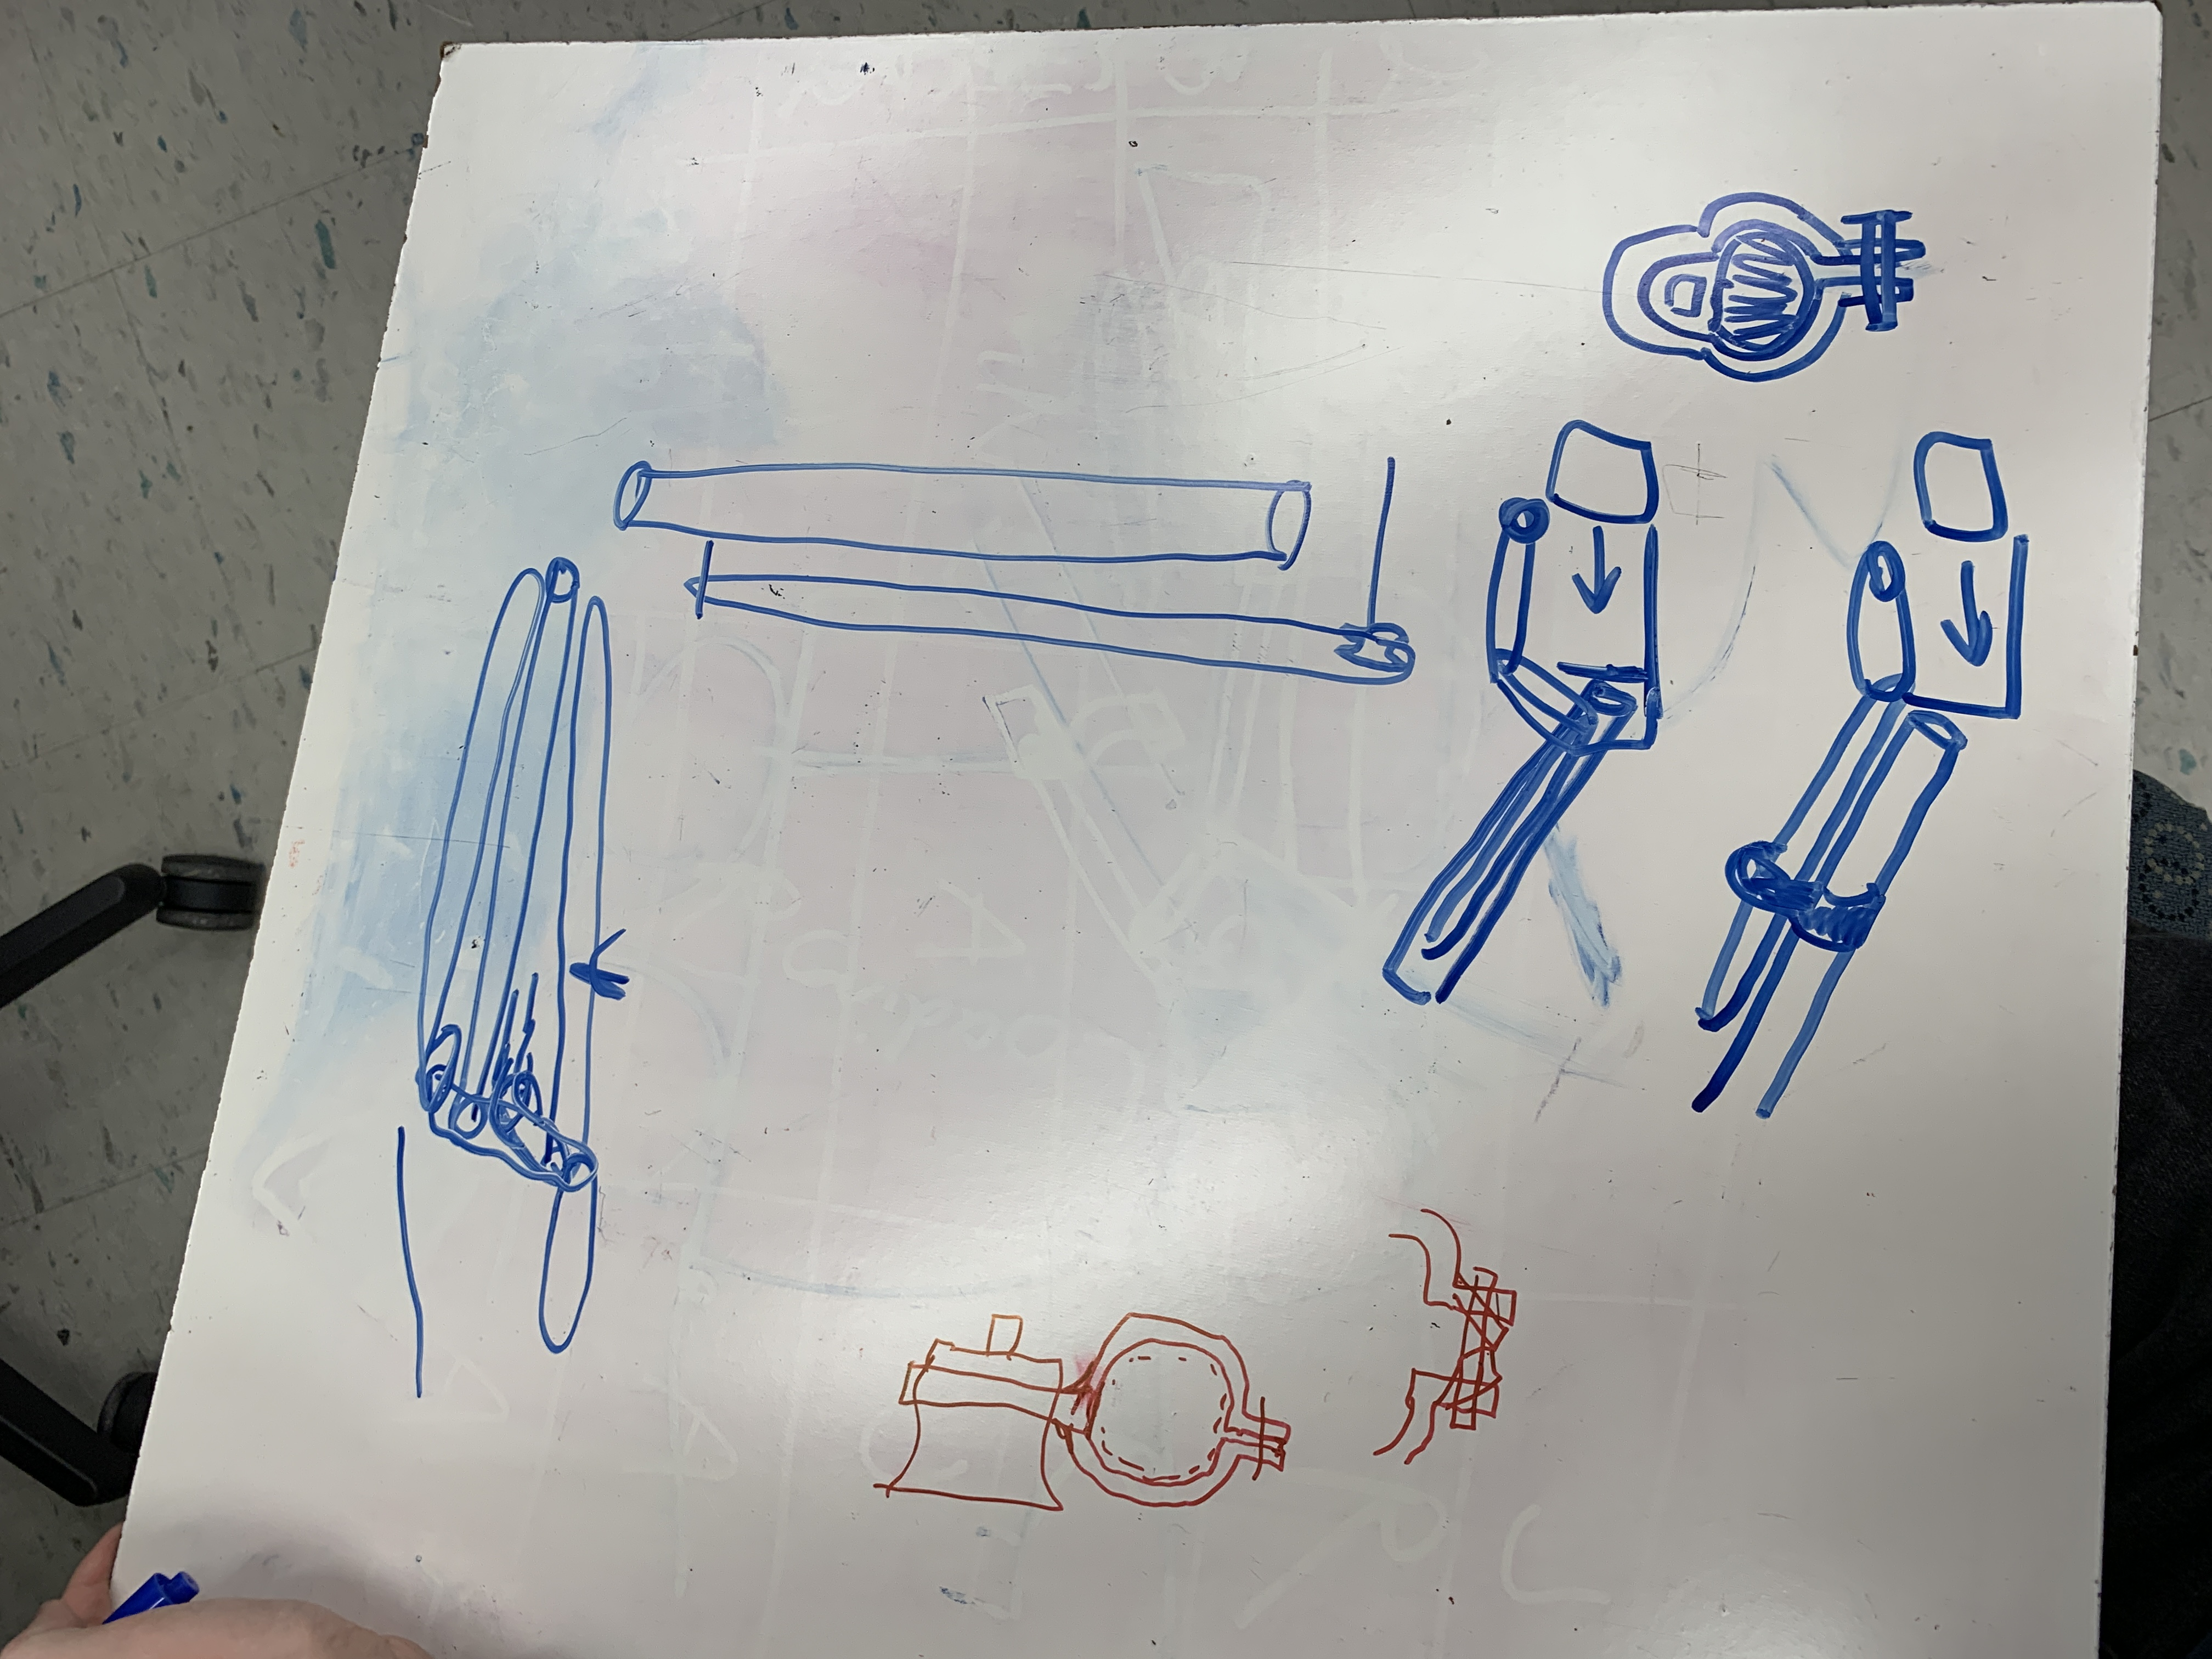
\includegraphics[width=0.95\textwidth]{Meetings/November/11-17-21/11-17-21_Hardware_Figure1 - Nathan Forrer.JPG}
  \caption{Various intake sketches}
  \label{fig:pic1}
\end{minipage}%
\hfill%
\begin{minipage}[b]{.48\textwidth}
  \centering
  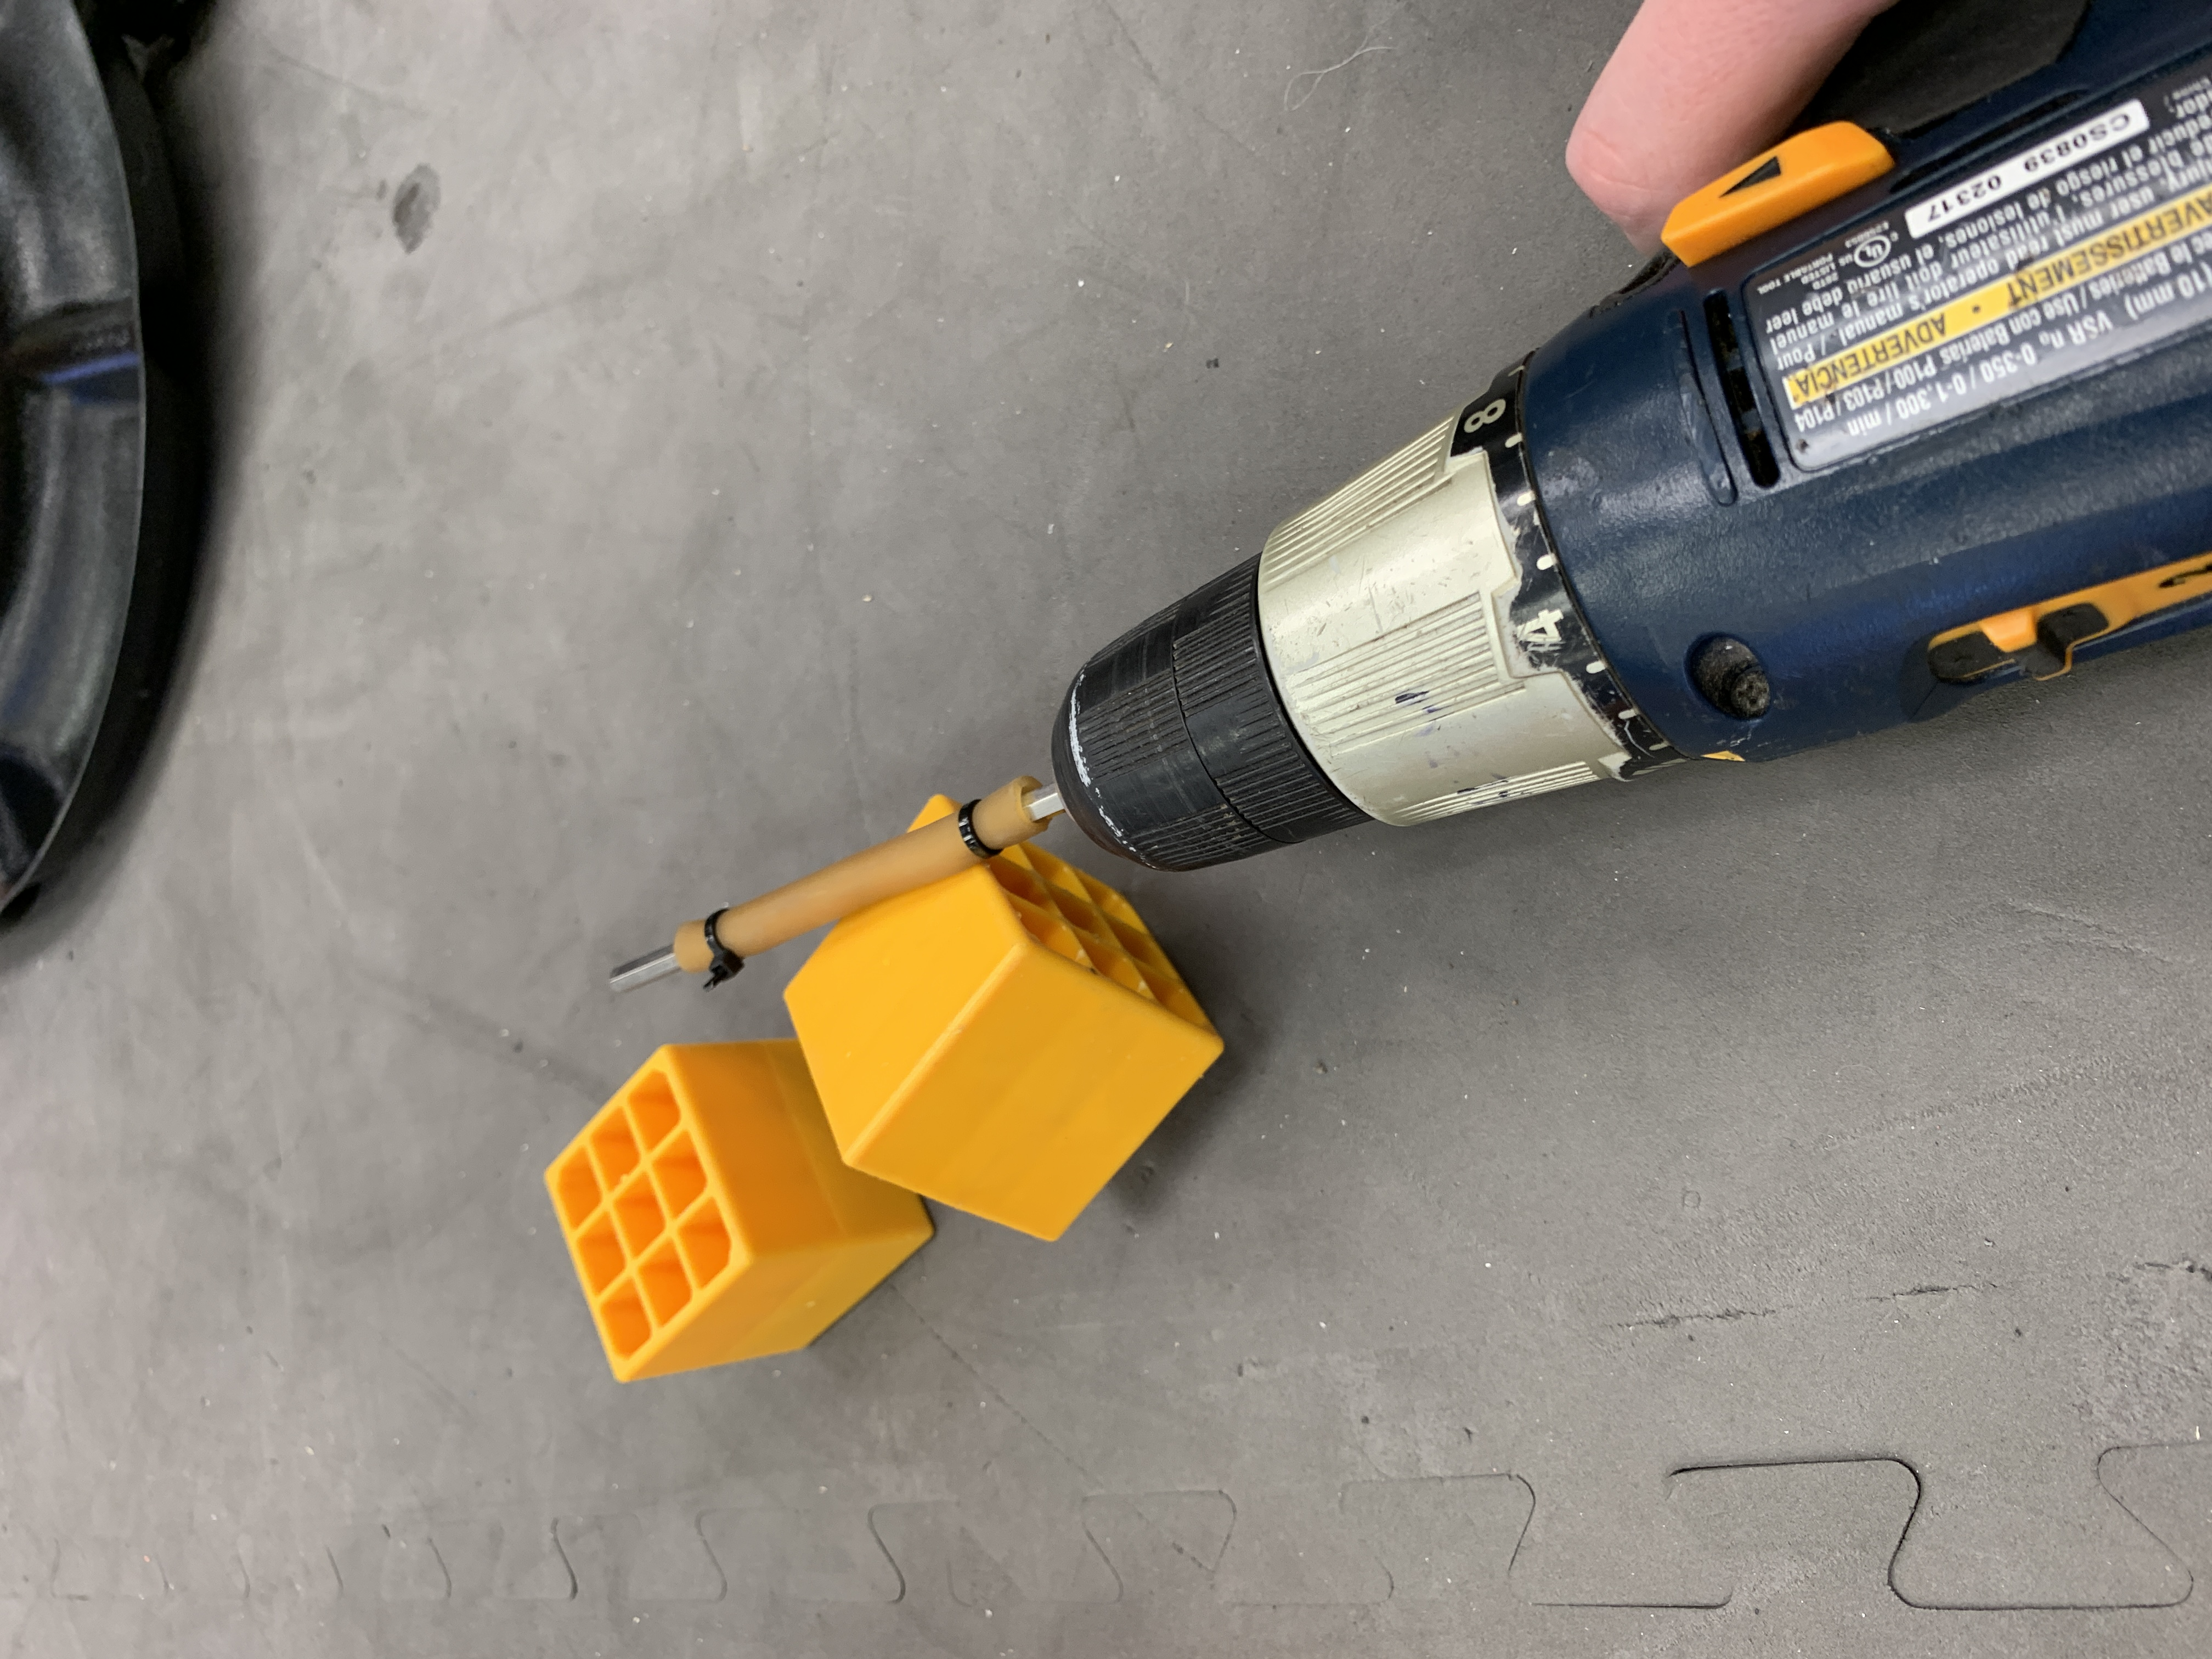
\includegraphics[width=0.95\textwidth]{Meetings/November/11-17-21/11-17-21_Hardware_Figure2 - Nathan Forrer.JPG}
  \caption{Prototyping a surgical tube roller}
  \label{fig:pic2}
\end{minipage}
\end{figure}


\whatsnext{
\begin{itemize}
    \item Design roller intake in CAD
\end{itemize} 
}

